\chapter{Фильтрация изображений с периодичностью}
\label{ch:chap1}

\definecolor{codegreen}{rgb}{0,0.5,0}
\definecolor{codegray}{rgb}{0.5,0.5,0.5}
\definecolor{codepurple}{rgb}{0.58,0,0.82}
\definecolor{backcolour}{rgb}{0.95,0.95,0.92}

\lstdefinestyle{mystyle}{
    backgroundcolor=\color{backcolour},   
    commentstyle=\color{codegreen},
    keywordstyle=\color{magenta},
    numberstyle=\tiny\color{codegray},
    stringstyle=\color{codepurple},
    basicstyle=\ttfamily\footnotesize,
    breakatwhitespace=false,         
    breaklines=true,                 
    captionpos=b,                    
    keepspaces=true,                 
    numbers=left,                    
    numbersep=5pt,                  
    showspaces=false,                
    showstringspaces=false,
    showtabs=false,                  
    tabsize=2
}

\lstset{style=mystyle}

Скачиваем какую-нибудь картинки с хорошо заметной периодичностью \href{https://drive.google.com/drive/folders/1oewu85taKvyxAUhXNH48ImTFtI1SpFag}{отсюда}, чтобы полечить её ниже.

\begin{figure}[ht]
    \centering
    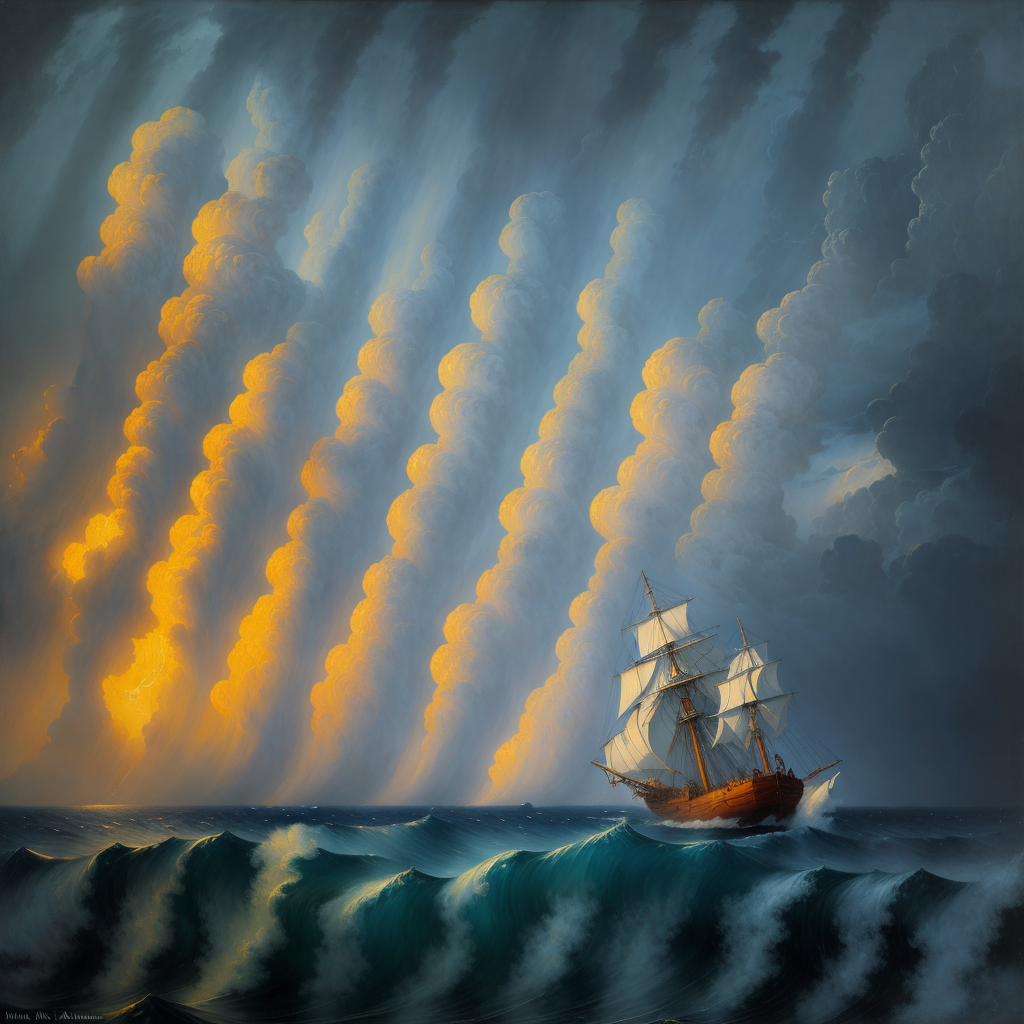
\includegraphics[width=0.5\textwidth]{ship.png}
	\caption{Оригинал}
\end{figure}
Теперь с помощью \texttt{MATLAB} функционала находим Фурье-образ нашего изображения, причём дабы сделать его более наглядным, он примет следующуюю формулу $log(1 + |\hat{X}|)$ :

\begin{figure}[ht]
    \centering
    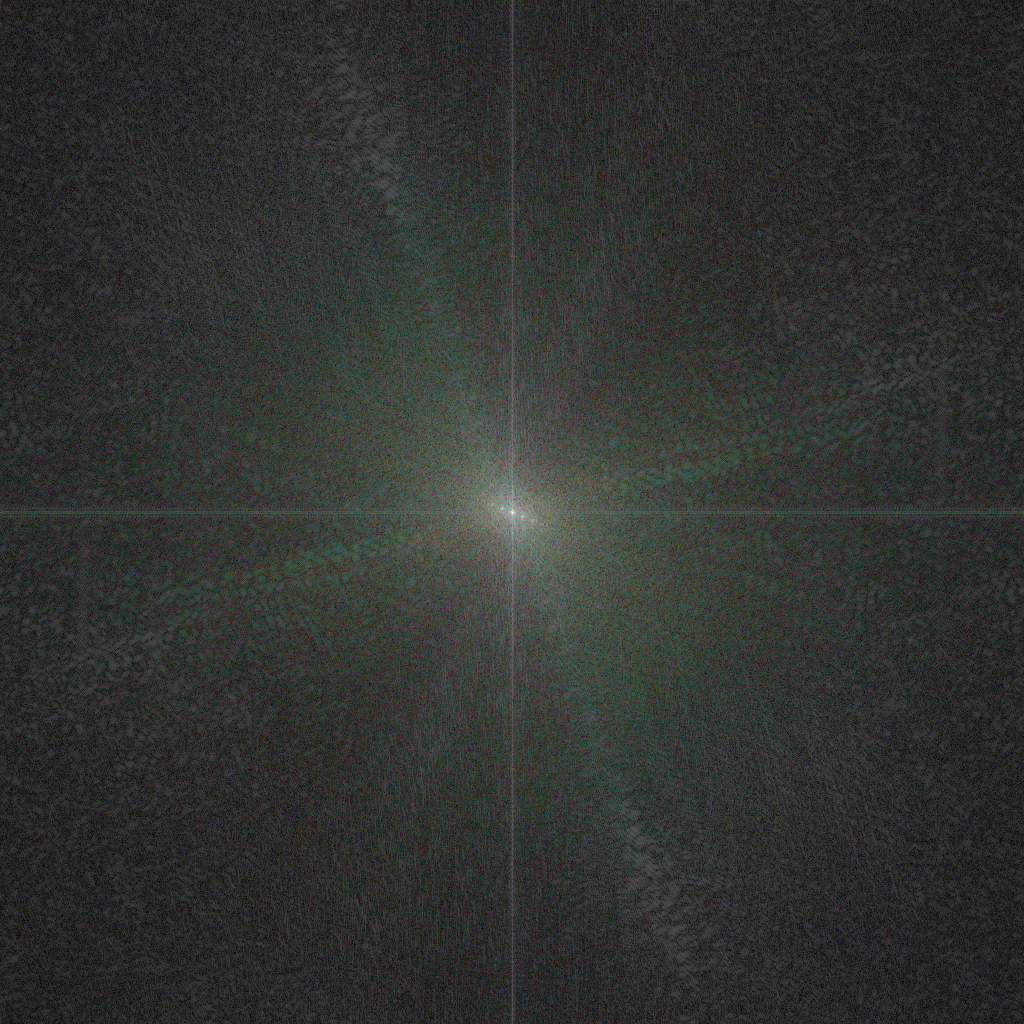
\includegraphics[width=0.5\textwidth]{FFT_IMAGE.png}
	\caption{2D Образ Фурье}
\end{figure}
\newpage
Понимать такое Фурье изображение следует так - чем ближе к краю изображения, тем более эти пиксели отвечают за краевые точки в изображении, "каркас" изображения. И наоборот, основные детали изображения заложены около центра образа.
В нашем случае мы должны искать пики около центра, потому что периодичность - это не "каркас" изображения, это детали. Вот что я выделил:
\begin{figure}[ht]
    \centering
    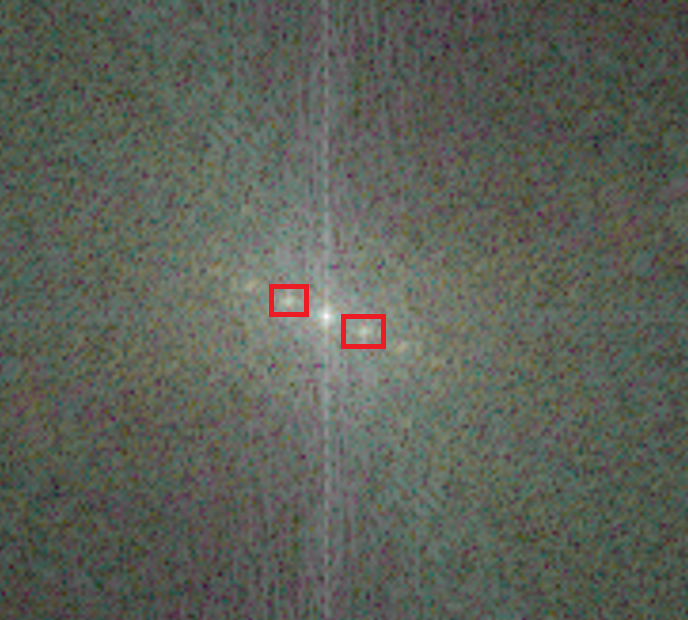
\includegraphics[width=0.5\textwidth]{FFT_IMAGE_peaks.png}
	\caption{Приближен центр - найденные пики (белые точки) }
\end{figure}


Для лучшей фильтрации, лучше воспользоваться инструментом Штамп из фотошопа, и аккуратно замазать эти два пика и рядом стоящие белые области,
 вот что получим после обратного преобразования:

\begin{figure}[ht]
	\centering
\hspace*{\fill}%
	\begin{subfigure}[b]{0.49\textwidth}
        \centering
		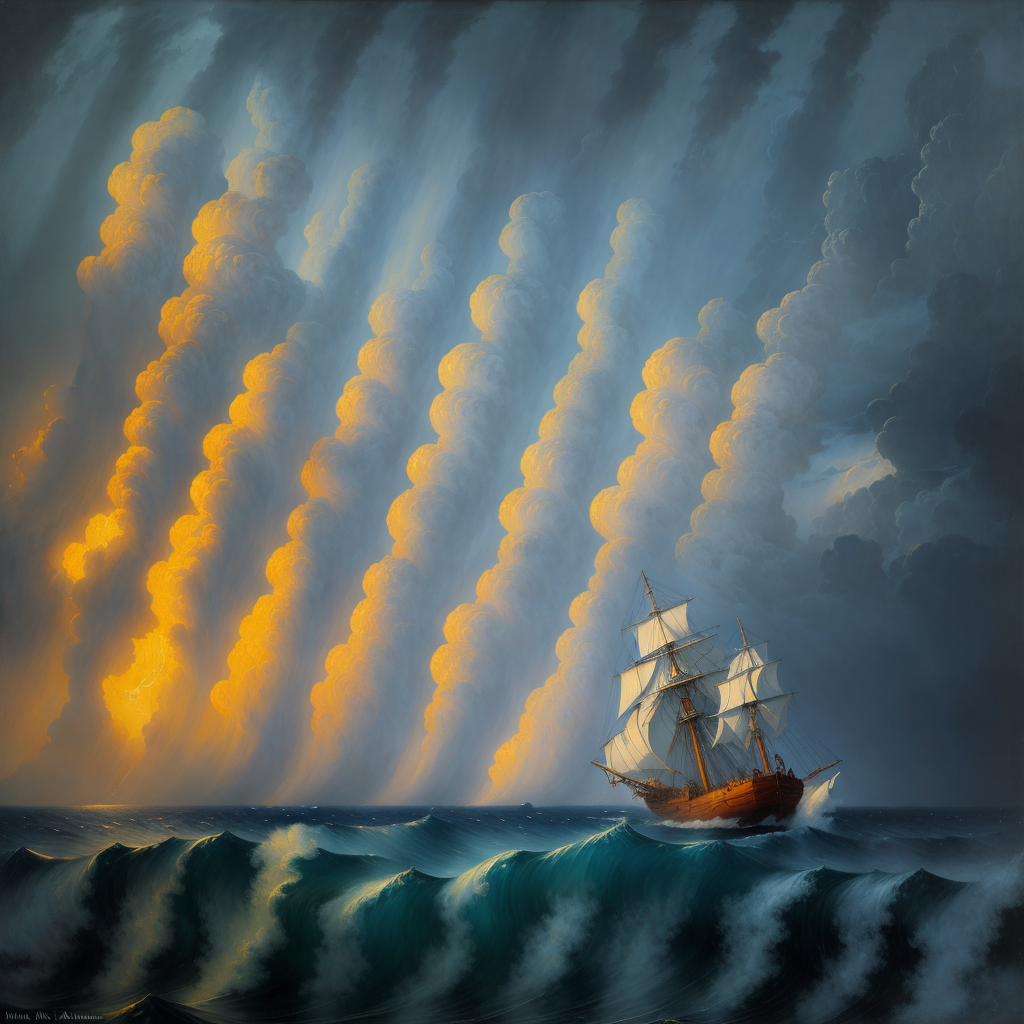
\includegraphics[height=5cm,keepaspectratio]{ship.png}
		\caption{Оригинал}
	\end{subfigure}
\hfill
	\begin{subfigure}[b]{0.49\textwidth}
        \centering
		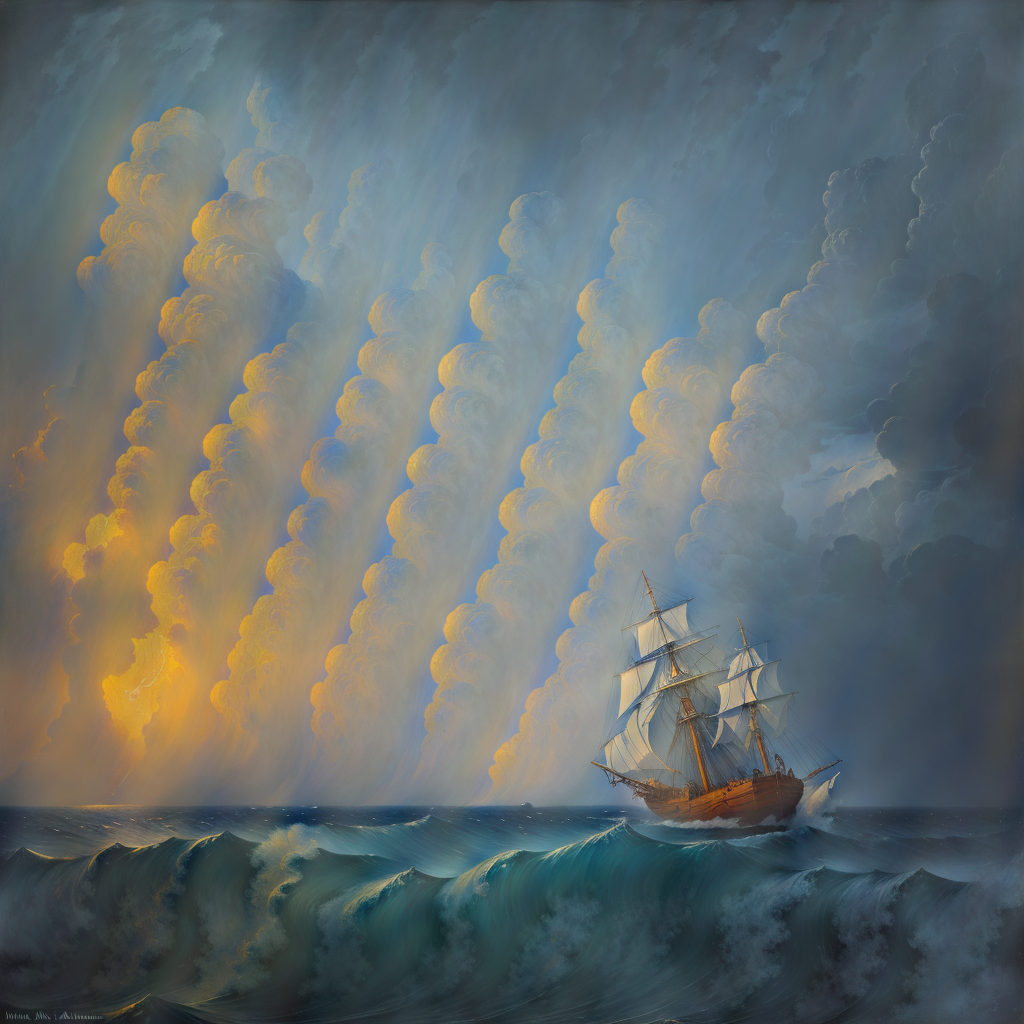
\includegraphics[height=5cm,keepaspectratio]{ship_restored.png}
        \caption{Почистили периодичность}
	\end{subfigure}
\hspace*{\fill}%
\end{figure}

И действительно, нам удалось убрать самую заметную периодичность, а значит фильтрация отработала хорошо.

\endinput